\chapter{Implementación}

\section{Volume Mapper}

Para poder visualizar un volumen con VTK mediante \textit{Direct Volume Rendering}, necesitamos un \textit{Volume Mapper}. La librería nos ofrece varias alternativas:
\begin{itemize}
	\item \texttt{vtkAMRVolumeMapper}
	\item \texttt{vtkFixedVolumeRayCastMapper}
	\item \texttt{vtkGPUVolumeRayCastMapper}
	\item \texttt{vtkSmartVolumeMapper}
	\item \texttt{vtkVolumeRayCastMapper}
	\item \texttt{vtkVolumeTextureMapper}
	\item \texttt{vtkVolumeTextureMapper3D}
\end{itemize}

Entre esta lista tenemos algunos que utilizan o texturas o \textit{ray casting}, o la CPU o la GPU. Pero hay uno que es especial con respecto al resto. Se trata de \texttt{vtkSmartVolumeMapper}.

Este \textit{Volume Mapper} es una versión mejorada del \texttt{vtkGPUVolumeRayCast Mapper} por lo que utiliza la GPU (si el dispositivo cuenta con una) y la técnica de \textit{ray casting}. Además cuenta con nuevas características con respecto al resto, como el poder definir infinitos planos de corte para poder ver el interior del volumen \cite{smart_volume_mapper}.

Por tanto, el \textit{Volume Mapper} utilizado será el \texttt{vtkSmartVolumeMapper}.

\section{Función de transferencia}

La función de transferencia es la encargada de dar a un valor de intensidad las propiedades de color y opacidad que le corresponden para la visualización del volumen.

En VTK la función de transferencia forma parte de la clase \texttt{vtkVolume Property}. Para ello proporciona otras dos clases:
\begin{itemize}
	\item \texttt{vtkColorTransferFunction}: Para definir el color. Se enlaza a \texttt{vtk VolumeProperty} con el método \texttt{SetColor}.
	\item \texttt{vtkPiecewiseFunction}: Para definir el color. Se enlaza a \texttt{vtkVolume Property} con el método \texttt{SetScalarOpacity}.
\end{itemize}

Podemos, por tanto, diferenciar dos partes fundamentales en la función de transferencia, la encargada de dar la propiedad de color y la de dar la propiedad de opacidad. Ambas trabajan de forma independiente. Es decir, cuando se define un punto en una de ellas, no tiene por qué definirse en la otra.

\subsection{Color}

Para definir esta función (\texttt{vtkColorTransferFunction}), hay que agregar puntos para valores de intensidad a los que se les asignará un color. VTK se encargará de interpolar entre un punto y otro (Figura \ref{fig:color_tf}). 

Por defecto, cuando no hay ningún punto, a todos los valores de intensidad les corresponderá un color negro. De forma parecida se comporta cuando solo hay un punto pero en lugar de negro, les corresponderá el color del punto que se ha definido.

VTK permite trabajar tanto con HSV como con RGB y para añadir un punto hay que utilizar \texttt{AddHSVPoint} o \texttt{AddRGBPoint}. A estos métodos se les pasa un primer parámetro en coma flotante con el valor de intensidad donde se establecerá ese punto y otros tres con las distintas exponentes (\textit{hue}, \textit{saturation}, \textit{brightness} o \textit{red}, \textit{green}, \textit{blue}).

\begin{figure}[H]
	\centering
	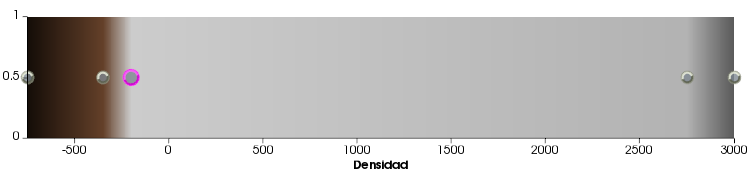
\includegraphics[width=10cm]{imagenes/color_tf}
	\caption{Parte de color de la función de transferencia del \textit{preset} \textit{CT-Cardiac} extraído del software Slicer \cite{slicer} donde se puede ver que hay 6 puntos definidos y los valores intermedios se obtienen interpolando}
	\label{fig:color_tf}
\end{figure}

\subsection{Opacidad}

Con el color no bastaría, pues si comprobásemos ahora añadiéndole tan solo el \texttt{vtkColorTransferFunction} al \texttt{vtkVolumeProperty} observaríamos que no se pinta nada en pantalla. Esto es porque por defecto, al no tener ningún punto la función de opacidad (\texttt{vtkPiecewiseFunction}) es una constante con valor 0 (transparente). 

Para definir esta función se trabaja de forma parecida a como se hace con el color, añadiendo puntos. El método que hay que utilizar es \texttt{AddPoint} al que se le pasan dos parámetros en coma flotante. El primero con el valor de intensidad y el segundo con la opacidad en ese punto. Para obtener los valores en puntos intermedios, se interpola entre los dos puntos en los que está. De forma que si para el valor de intensidad 100 hemos definido una opacidad de 0.5 y para el de 200 1, al valor de intensidad 150 le corresponderá 0.75.

Combinando color y opacidad podemos obtener la función de transferencia para nuestro volumen (Figura \ref{fig:opacity_tf}). 

\begin{figure}[H]
	\centering
	
\includegraphics[width=10cm]{imagenes/opacity_tf}
	\caption{Función de transferencia del \textit{preset} \textit{CT-Cardiac} extraído del software Slicer \cite{slicer}. Se pueden ver los cuatro puntos que definen la función de opacidad y de fondo la función de color anterior}
	\label{fig:opacity_tf}
\end{figure}
